\title{Artificial Life - Final Project Report: Implementing the Rosen Diagram}
\author{Ryan Spangler}
\date{\today}

\documentclass[12pt]{article}

\usepackage{commath}
\usepackage{graphicx}
\usepackage{listings}
\usepackage{amsfonts}

% python highlighting ----------
\usepackage{color}
\usepackage{listings}
\usepackage{textcomp}
\usepackage{setspace}
%\usepackage{palatino}

% \doublespacing

\setcounter{secnumdepth}{0}

\begin{document}
\maketitle

\section{Abstract}

In response to Rosen's attempt to formalize the organism as a category theoretical diagram \cite{Rosen}, I attempt to build an instantiation of his metabolic-repair system as a trio of mutually modifying executable trees.  These trees incorporate a sense of entropy and renewal to bring the dynamics of the diagram to life in the face of a supplied generative environment.

\section{Introduction}

What is life?  This question has been asked many times, in countless forms.  It is hard to approach for many reasons: the inherent complexity of life, the dizzying variety of life's forms, the immense physical scale living things span, the tangled mess of feedback loops and reciprocities in even the simplest organisms.  The interplay of evolution and development is a riddle even the sphinx would balk at \cite{Oyama}.  

Yet as long as there is something unknown, not yet understood, people will throw themselves at the problem until the mystery has been cracked.  Just as in physics, we seek a universal solution, a succinct description or kernel that will unfold into the bewildering variety we witness.  Just as Newton's laws of gravitation provided a means for us to turn the subtle motions of the stars and celestial bodies into a single set of relationships, we long for a formalized account of biological processes, that makes the task of approaching and understanding the wide array of biological systems a tractable one.  

Beyond that, we all sense there is a unifying principle behind life.  We can *feel* it, we are instances of life ourselves.  We can immediately apprehend the living from the dead, it is obvious to discern.  It is the defining that is elusive.  

This issue of defining life is actually inseparable from the issue of making models of anything.  Modeling is how we understand the world that we can never directly experience.  A model is a substitute, a stand-in for some real world phenomenon or system we are actually interested in.  A model is useful in as much as we can perturb the model and its resulting behavior reflects the behavior of the system it was intended to model.  

In physics we build our models out of equations defining relationships between various measurable quantities.  Newton provided us with models of celestial dynamics specifically, but beyond that, and more implicitly, he provided us a general framework for defining models.  His models were such a wild success at the time people started trying to apply the same ideas to everything.  To this day, his implicit structure of defining models is still in use, still guiding the way we think about translating a natural system into a formal one.  Physics has moved on, from relativity to quantum mechanics to present day, with more and more complex models to describe the continuous revelations provided by experiment, but it is still using the same basic structure of entailment.  It is this entailment structure that has been tried, and failed, to be applied to biological systems.  Is it merely that the right model has not been found?  Or is there some deeper limitation in what kinds of models we are trying to apply to biological phenomena?

Rosen claims that there is an inherent flaw in attempting to apply the Newtonian entailment structure to biological systems \cite{Rosen}.  Specifically, Newtonian models define how one moment is translated to the next.  This is the only mode of entailment: one moment implies the next.  However, the function F which translates the previous state to the next does not change, it is static across all moments.  The states form a one-dimensional chain that can be infinitely extended by iteratively applying the universal transformation F.  It is this F that defines the system, and unearthing the F which governs the behavior of the whole universe is the main goal of physics.  

\begin{center}
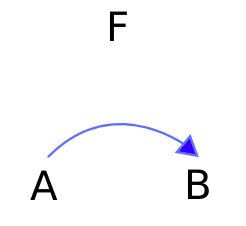
\includegraphics[scale=0.6]{newton.png}
\end{center}

In Rosen's world, F is not static.  Organisms form a closed causal loop where everything is entailed by something else within the system, including the transformation itself.  His main claim is that organisms are not modelable by chains of states governed by a static transformation.  Any transformation must itself be entailed by another transformation, which itself is generated by yet another transformation.  His full diagram is as follows:

\begin{center}
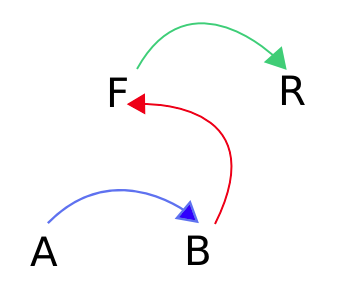
\includegraphics[scale=0.6]{rosen.png}
\end{center}

In this diagram, A (here called E) entails B through F (here called M) just like in Newton's model, but M itself is entailed by B from R.  R is generated from M by B.  In Rosen's terminology, M corresponds to ``metabolism'', that which generates B, and R maps to ``repair'', that which renews M.  E acts as the environment, an unentailed element which embodies the idea that an organism is an open system interacting with external forces beyond its membrane.  The three main functions are all entailed by other functions which are part of the system.  All the transformations act as both effector and effectee, as actor and acted-upon.  It is this diagram that I have attempted to implement for this project.

\section{Methods}

Many considerations were necessary in order to implement a system that behaves in a way representative of the diagram.  The main issue is that whatever F, B and R are, they must have the capacity to alter or influence the other elements, as well as the ability to be altered.  Specifically, there are three roles each element must play.  It must be an actor/function/transformation, taking elements from one domain into another.  Second, it must be readable, that is, a source or raw material for the transformation to work on.  Third, it must be generatable by the transformation operating on the previous element.  

What kinds of things have this structure?  A matrix can act as both a function (linear transformation at least) and data, in that it is simply a grid of numbers, so that would fulfill the requirement.  In my case though I chose to use abstract executable trees.  

A program can be thought of as a tree of instructions, with the root being the first instruction and execution taking a single path from root to leaf.  Each node is a particular operation and the branches from that node are conditional paths of execution.  So the tree only branches during conditional operations, otherwise it performs the operation of its node and continues along whatever execution path is given by its single child.  During a conditional operation the branch of execution is determined by the outcome of whatever predicate is associated with the operation.  

\begin{center}
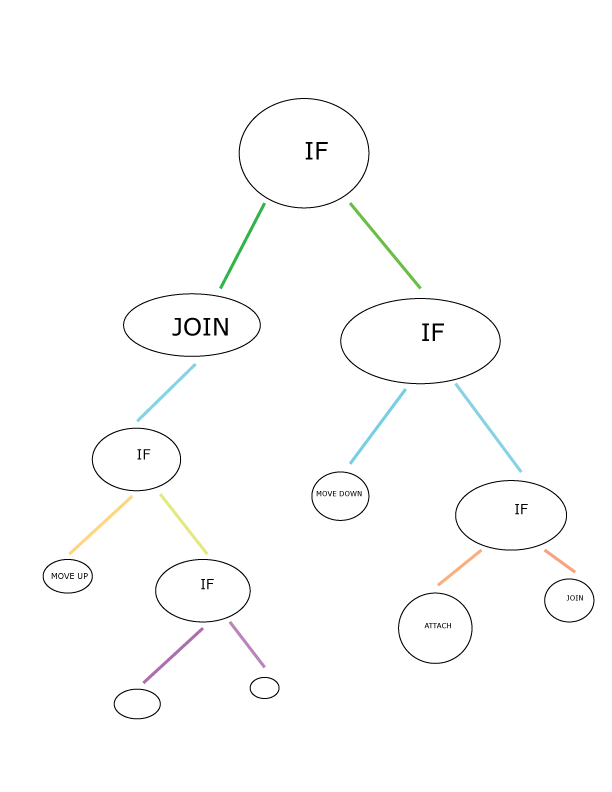
\includegraphics[scale=0.6]{treerainbow.png}
\end{center}

In this case, the operations in each node work on trees themselves, rendering each tree a program that operates on other trees.  Each tree holds iterators to both a focus and a target tree.  The focus is a node inside another tree that is currently being read: the 'A' in the diagram.   The target is indexing a node into a tree that is being altered: the 'B' in the diagram.  When the tree executes, a single execution path is chosen based on evaluating the conditions in each 'if' node as it is reached.  This execution path has operations that read from the focus tree and writes to or alters the target tree.  In the case of 'F', the conditions depend on the particular properties of the environment 'A', which can be defined according to whatever application the diagram is being implemented for.  In this way I tried to make the system general in that the environment can be defined in any way.  As long as you supply the operations which work on the environment and a function which generates values from the environment, it can correspond to whatever you want.  

For these tree operations I chose a limited set of operators: move, grow, renew, and if.  The move operators are for navigating up and down the focus and target trees.  So there is a corresponding operator for moving up the focus tree as well as moving up the target tree, as well as for down.  If the iterator for that tree is already at the top when execution encounters a move up operator, nothing happens.  Likewise with move down.  

The grow operator takes the element the iterator is pointing to in the focus tree and adds it to the target node in the target tree. The grow operation attempts to fill out the tree, but when the tree is full it attaches it as a subtree of the node to be added, growing the tree from the root down.  This is to offset the purging which occurs from bottom up.  So there is a kind of cyclical adding and purging that flows from root to leaf, constantly renewing the operations that compose its functional identity.

The renew operator relates to the idea of entropy.  In the discussion of the relationship between various components in an organism, a key idea is that in the working of metabolism translating elements of the environment into energetic bonds, the actual structure of the metabolic components break down.  There is no perpetual motion machine, in order for these molecules to function they are continually expending energy and compromising their basic structure in order to carry out their tasks.  This damage to the basic components of metabolism must be offset by a process.  This process of renewal of the metabolic actors is what Rosen called the ``repair'' function, and is represented by 'R' in the diagram.  

In order to incorporate this idea of wear and renewal into this system I added in a value to each node called ``passes'', which keeps track of every time this node is visited during execution.  If the node is  a leaf and its number of passes exceeds some limit, the node is removed from the tree.  In this way the trees are progressively pruned during their operation based on how heavily the nodes are used in execution.  The renew operator then removes the wear from its target node, but at the expense of wear on itself.  This attempts to keep a balance between the proliferation of new nodes through attachments and insertions and a need to remove nodes through a kind of simulaed entropy.  However, it is a form of imposed entropy, not innate entropy as we witness in physical systems.  This is one of the greatest differences between physical systems and simulated ones, is that in physical systems entropy is an unavoidable quality of natural processes, imposed by the universe, whereas in simulated systems entropy must be inserted.  This is important because much of what organisms do can be considered in relation or opposition to entropy, so any simulated organism by necessity is working under a contrived set of the real laws of nature which spurned its existence in the first place.  

The if operator branches execution depending on what the type of node it is looking at in the focus tree.  Each if compares this type to its own internal type, so each if is a recognizer of only one type of node.  If these types match, it goes down the first branch.  Otherwise, it heads down the second.

\section{Experiments}

Many experiments were run.  The first trees I built were far more complicated than the final ones:  more conditions, more outlets, complex purging rules etc.  As I went I pared down the set of operations to only the four described above.  There were a number of different ways to join or splice in nodes that proved unnecessarily complicated.  Also, there was a set of conditions for every type of operation:  moving up in the target tree vs moving up in the focus tree for instance.  This proliferation meant that all of the if operations were overly specific and rarely traveled down the path corresponding to a 'true' condition.  Making the conditions agnostic to the more refined details of each operator gave a higher positive response and a more varied behavior from the system.  

Another important distinction was between whether nodes should grow from the top or the bottom.  I had assumed that I would just add nodes as leaves, but in practice this meant that the leaves that were just added were also the first removed by the purging process.  This lead to a situation where there was a large static clump towards the root with many subtrees flitting in and out of existence further down the tree.  For another flavor I gave conditions where the node could be added as the root.  This gave more of an effect of continual renewal, where functional components come into being and then migrate down the tree until they are eventually removed through purging.  This lead to a much more organic feel in the growth of the trees, with all nodes going through a similar life cycle.  

One key point about all of the experiments I ran is that I modeled the environment as a stochastic element.  The M tree based its conditions on a mapping between a value from 0 to 1 and a type of tree node.  In the future I would like to model a real environment, and also provide operations that in turn acted upon the environment, closing the causal loop and simulating something resembling a real system.  

\section{Results}

The results are nothing approaching conclusive.  This was more of an exploration than a real scientific study, I wanted to see what kind of system I could build that would emulate the relationships defined in the Rosen diagram.  Nonetheless, there are products of this endeavor.  Here is a snippet of code from one of the trees being generated on the fly from its relationships with other trees:

\begin{center}
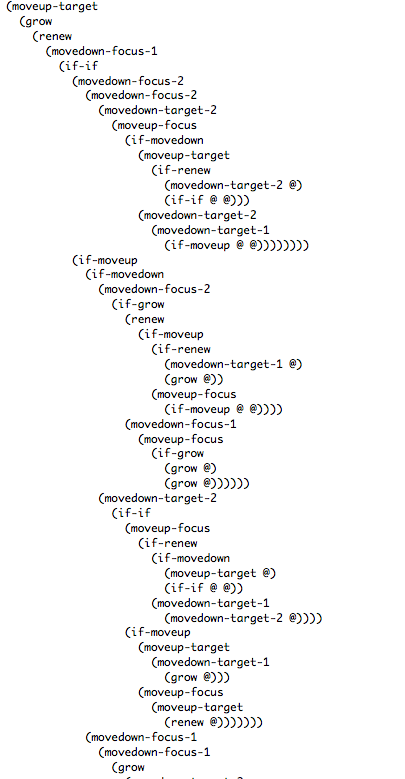
\includegraphics[scale=0.6]{treecode.png}
\end{center}

And here is a screenshot of the simulation in action.  Trees are growing and shrinking, their functional dynamics elaborated and refined continuously:

\begin{center}
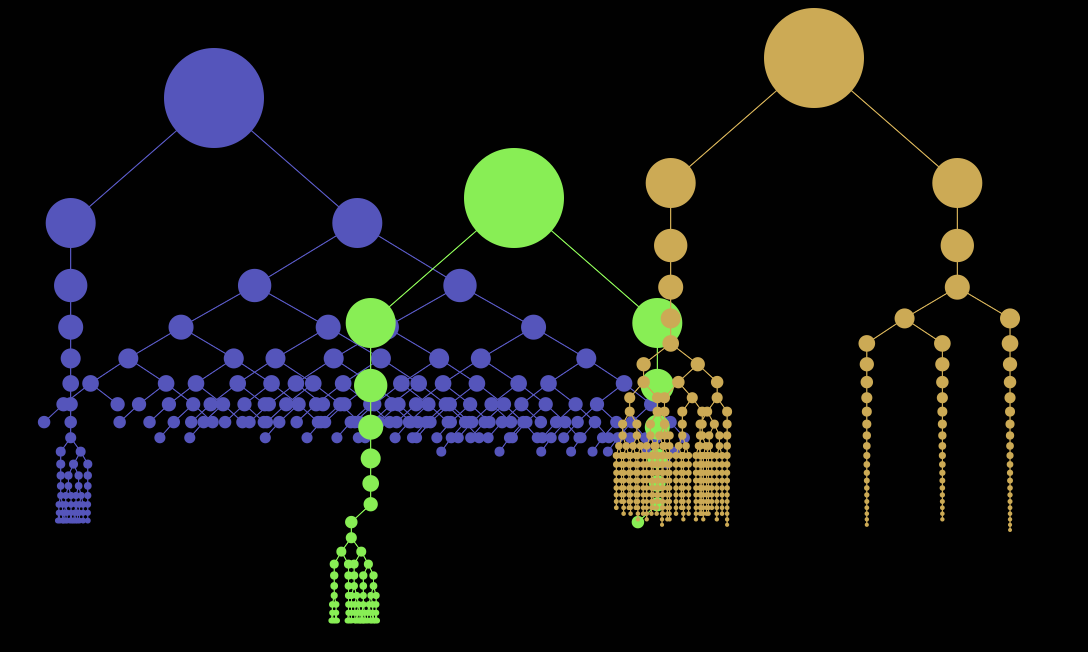
\includegraphics[scale=0.4]{treegrowth.png}
\end{center}

To really get any results I would have to hook it up to a real environment and provide it with meaningful input.  This is a project for the future.

\section{Discussion}

Much of what Rosen spoke of was that by the nature of an organism it incorporates all of its physical existence into the perpetuation of that form \cite{Alon}.  This situation is inherently unsimulatable, to produce a *genuine* organism one would have to sincerely create such a system in materio.  However, this does not mean there cannot be useful simulations constructed in the spirit of biological dynamics.  Indeed, possibly by crossing the levels here of what is executing and what is executed on, we are creating a new bottom where synthetic organisms could flourish.  

The other consideration is that as a consequence of their physical embodiment, entropy is a key force behind the activity of the organism on a day to day basis \cite{Ho}.  The continual wearing down of the engines of life must be offset by some kind of process of renewal if the organism is going to last a day.  In the physical world this source of entropy is inherent, and the sole source of meaning behind the things organisms do.  The process of living is harnessing entropy to defy entropy, to turn the gradient of entropy around on itself and use it to actually sustain the form, rather than destroy it.  This is done of course with a continual flow of energy, without which nothing could live.  In a simulation, can it be meaningful if entropy must be supplied, as if it is another parameter?  Can a simulation be built that actually exhibits entropy as a necessary consequence of its functioning, and thereby provides a more solid foundation for replicating the dynamics particular to life?  Without some kind of embodiment of entropy, as a metaphor or model or otherwise, work cannot even begin on building something whose behavior is defined in terms of, and in response to entropy.

\section{Conclusion}

Rosen's work is fundamental in an important way:  he examined the underpinnings of our mutual assumed epistemology, and rejected a particular assumption about how we understand reality in a formal context.  By showing that there are other kinds of models that can be built, with a richer set of structural entailments, he was providing us with options we didn't know we required.  Beyond that, he showed us that there is a wealth of fresh perspective to be found by challenging hidden assumptions, and points towards a way forward in constructing models that are rich enough, robust enough, flexible enough to truly capture the overall process of living.  This work was a first foray into making something concrete out of it.  It was utterly a programmer's literal take on what is a more general idea, and I have gained much insight into what Rosen may have really meant by these three functional components (plus environment!).  Perhaps rather than explicit functions, these three elements are more components of a single thing, or perspectives on the same thing, which happen to have this mutual relationship of entailments between them.  Perhaps with a deeper and more subtle understanding I will be able to apply these ideas in a more realistic context, now that I have gone this far.

\bibliographystyle{plain}
\bibliography{finalreport}

\end{document}  

